
The DHT (\ref{eq:DHT}) can be written equivalently as a matrix-vector product with $\mtx{A} \in \R^{m \times n}$
\begin{equation}
    \vct{g} = \mtx{A}\vct{f}, \qquad \mtx{A}(j,k) = J_0(\omega_j r_k).
\end{equation}


Show matrix arising from DHT, draw bands, say what happens in each region: local
expansion, direct, asymptotic, and why the local expansion can be accelerated

\begin{figure}
  \centering
  \begin{subfigure}[b]{0.45\textwidth}
    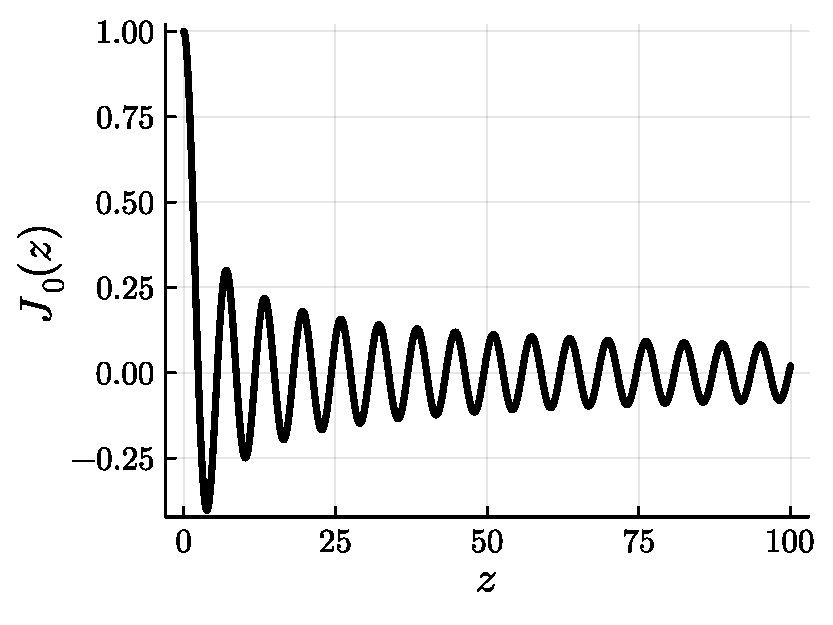
\includegraphics[width=\textwidth]{./figures/bessel_function.pdf}
  \end{subfigure}
  \begin{subfigure}[b]{0.45\textwidth}
    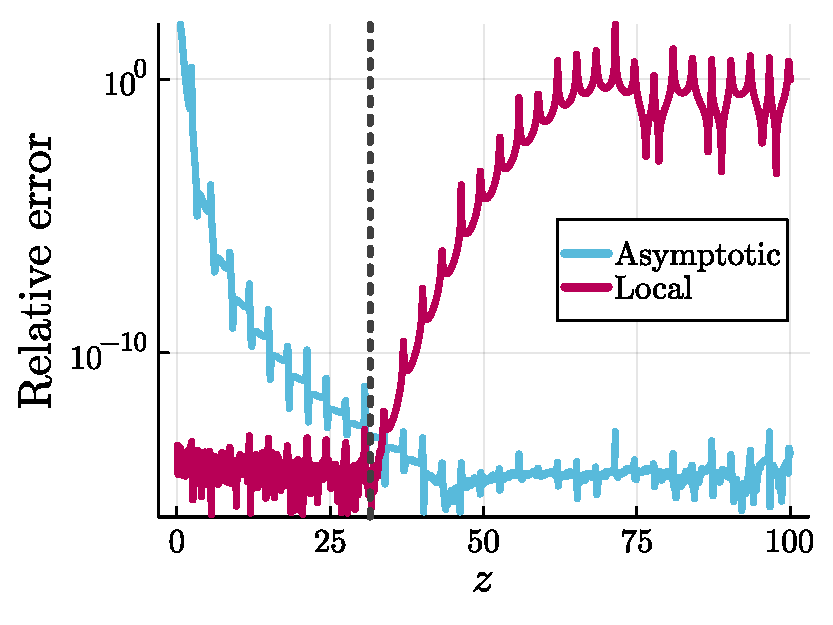
\includegraphics[width=\textwidth]{./figures/pointwise_errors.pdf}
  \end{subfigure}
  \caption{Bessel function $J_0(z)$ and pointwise relative error in approximating $J_0(z)$ using local and asymptotic expansions. Dotted vertical line shows crossover point where both expansions are accurate to $\epsilon = 10^{-12}$.}
\end{figure}

\begin{figure}
  \centering
  \newcommand\twa{0.29cm}
  \newcommand\tw{0.43cm}
  \begin{subfigure}[b]{0.23\textwidth}
    
\includegraphics[width=\textwidth, trim={\twa, \twa, \twa, \twa}, clip]{./figures/splitting.pdf}
    \caption{}
  \end{subfigure}
  \hfill
  \begin{subfigure}[b]{0.23\textwidth}
    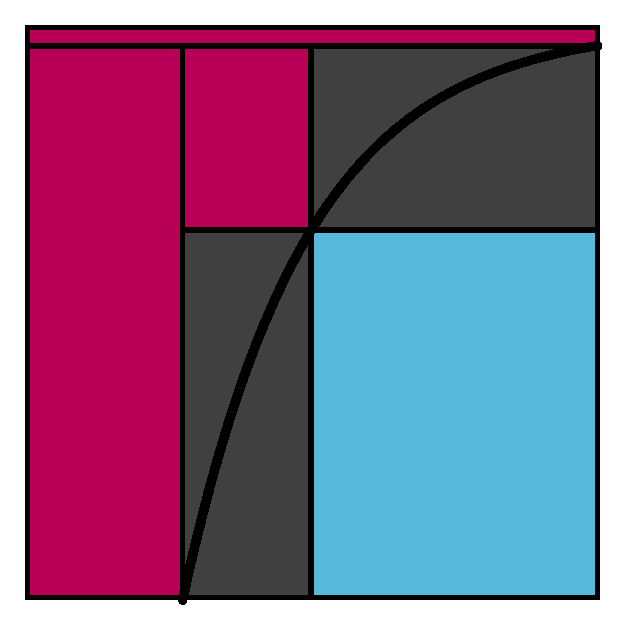
\includegraphics[width=\textwidth, trim={\tw, \tw, \tw, \tw}, clip]{./figures/splitting_lvl1.pdf}
    \caption{Level 1}
  \end{subfigure}
  \hfill
  \begin{subfigure}[b]{0.23\textwidth}
    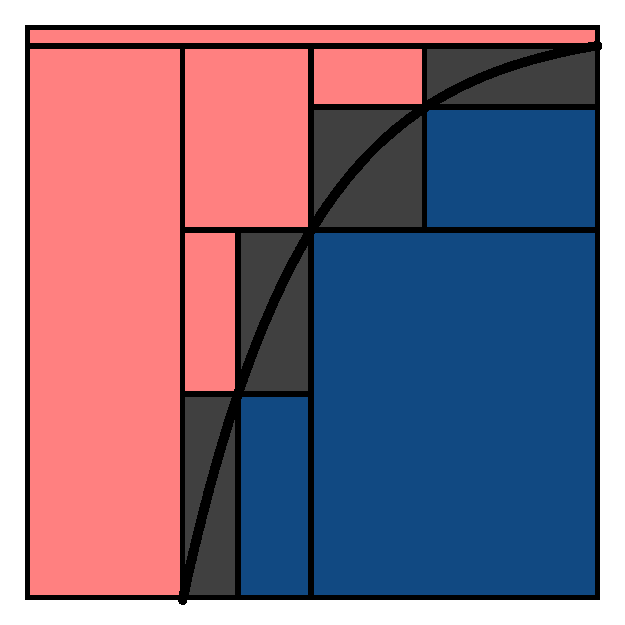
\includegraphics[width=\textwidth, trim={\tw, \tw, \tw, \tw}, clip]{./figures/splitting_lvl2.pdf}
    \caption{Level 2}
  \end{subfigure}
  \hfill
  \begin{subfigure}[b]{0.23\textwidth}
    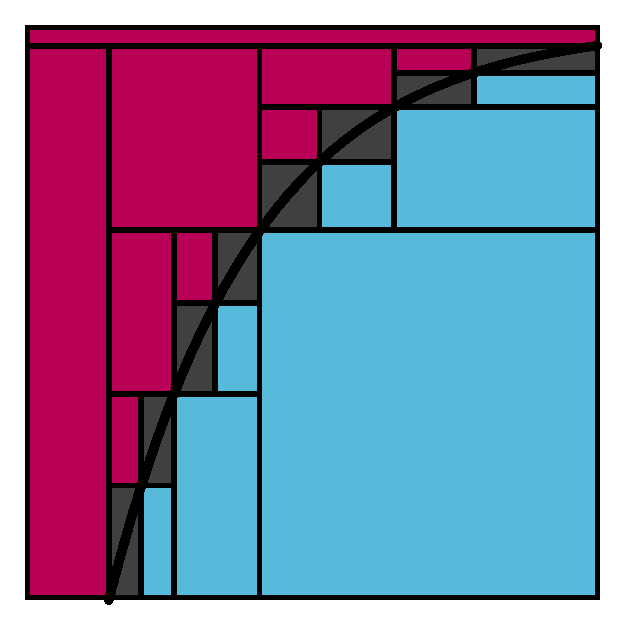
\includegraphics[width=\textwidth, trim={\tw, \tw, \tw, \tw}, clip]{./figures/splitting_lvl3.pdf}
    \caption{Level 3}
  \end{subfigure}
  \caption{Splitting of Hankel transform matrix $\bm{A}$ into local and asymptotic entries, and adaptive subdivision of $\bm{A}$ into corresponding sub-blocks by expansion.}
\end{figure}